% -*- latex -*-

\documentclass{article}

\usepackage{amsfonts}
\usepackage{amssymb}
\usepackage{amsmath}
\usepackage{graphicx}
\usepackage{subfig}
\usepackage{varioref}
\usepackage{fancyvrb}
\usepackage{ifthen}
\usepackage{cite}
\usepackage{xspace}
\usepackage{hyperref}

\usepackage{color}
\definecolor{yellow}{rgb}{1,1,0}
\definecolor{black}{rgb}{0,0,0}
\definecolor{ltcyan}{rgb}{.75,1,1}
\definecolor{blue}{rgb}{0,0,1}
\definecolor{red}{rgb}{1,0,0}
\definecolor{darkred}{rgb}{0.5,0,0}
\definecolor{darkgreen}{rgb}{0,0.5,0}

% Cite commands I use to abstract away the different ways to reference an
% entry in the bibliography (superscripts, numbers, dates, or author
% abbreviations).  \scite is a short cite that is used immediately after
% when the authors are mentioned.  \lcite is a full citation that is used
% anywhere.  Both should be used right next to the text being cited without
% any spacing.
\newcommand*{\lcite}[1]{~\cite{#1}}
\newcommand*{\scite}[1]{~\cite{#1}}

\newcommand*{\keyterm}[1]{\emph{#1}}

\newcommand{\etal}{et al.}

\newcommand{\fix}[1]{{\color{red}\textbf{\textsc{[#1]}}}}

\newenvironment{packeditemize}{
  \begin{itemize}
    \setlength{\topsep}{0pt}
    \setlength{\itemsep}{0pt}
    \setlength{\parskip}{0pt}
    \setlength{\parsep}{0pt}
    \setlength{\partopsep}{0pt}
}{
  \end{itemize}
}

\newenvironment{packeddescription}{
  \begin{description}
    \setlength{\topsep}{0pt}
    \setlength{\itemsep}{0pt}
    \setlength{\parskip}{0pt}
    \setlength{\parsep}{0pt}
    \setlength{\partopsep}{0pt}
}{
  \end{description}
}

% Avoid putting figures on their own page.
\renewcommand{\textfraction}{0.05}
\renewcommand{\topfraction}{0.95}
\renewcommand{\bottomfraction}{0.5}

% Make sure this is big enough so that only big figures end up on their own
% page but small enough so that if a figure does have to be on its own
% page, it won't push everything to the bottom because it's not big enough
% to have its own page.
\renewcommand{\floatpagefraction}{.75}

\title{Modern Visualization Pipelines}

\author{Kenneth Moreland}

\date{}

\sloppy

\begin{document}

\maketitle


\section*{Abstract}

The most common abstraction used by visualization libraries and
applications today is what is known as the visualization pipeline.  The
visualization pipeline provides a mechanism to encapsulate algorithms and
then couple them together in a variety of ways.  The visualization pipeline
has been in existence for over twenty years, and over this time many
variations and improvements have been proposed.  This paper provides a
literature review of the most prevalent features of visualization pipelines
and some of the most recent research directions.


\section{Introduction}
\label{sec:Introduction}

The field of scientific visualization was launched with the 1987 National
Science Foundation Visualization in Scientific Computing workshop
report\lcite{ViSC1987}, and some of the first proposed frameworks used a
\keyterm{visualization pipeline} for managing the ingestion,
transformation, display, and recording of
data\lcite{Haeberli1988,Lucas1992}.  The combination of simplicity and
power makes the visualization pipeline still the most prevalent metaphor
encountered today.

The visualization pipeline provides the key
structure in many visualization development systems such as the
Visualization Toolkit (VTK)\lcite{VTK}, SCIRun\lcite{SCIRun}, the
Application Visualization System (AVS)\lcite{AVS}, OpenDX\lcite{OpenDX},
and Iris Explorer\lcite{IRISExplorer}.  Visualization applications like
ParaView\lcite{ParaView}, VisTrails\lcite{VisTrails}, and
MayaVi\lcite{MayaVi} allow end users to build visualization pipelines with
graphical user interface representations.  The visualization pipeline is
also used internally in a number of other applications including
VisIt\lcite{VisIt}, VolView\lcite{VolView}, OsiriX\lcite{OsiriX}, 3D
Slicer\lcite{3DSlicer}, and BioImageXD\lcite{BioImageXD}.

In this paper we review the visualization pipeline.  We begin with a basic
description of what the visualization pipeline is and then move to
advancements introduced over the years and current research.


\section{Basic Visualization Pipelines}
\label{sec:BasicVisualizationPipelines}

A visualization pipeline encapsulates an algorithm in one of three types of
objects: \keyterm{sources}, \keyterm{filters}, and \keyterm{sinks}.  A
source object produces data that it makes available through an
\keyterm{output}.  File readers and synthetic data generators are typical
source objects.  A sink object accepts data through an \keyterm{input} and
performs an operation with no further result (as far as the pipeline is
concerned).  Typical sinks are file writers and rendering components that
provide images to a user interface.  A filter object has at least one input
from which it transform data and provides results through at least one
output.

The intention is to encapsulate algorithms in interchangeable source,
filter, and sink components with generic connection ports (inputs and
outputs).  An output from one component can be connected to the input from
another component such that the results of one algorithm become the inputs
to another algorithm.  These connected components form a
\keyterm{pipeline}.  Figure~\ref{fig:SimplePipeline} demonstrates a simple
but common pipeline featuring a file reader (source), an isosurface
generator\lcite{Lorensen1987} (filter), and an image renderer (sink).

\begin{figure}[htbp]
  \centering
  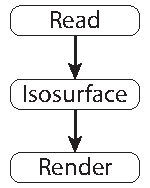
\includegraphics{images/SimplePipeline}
  \caption{A simple visualization pipeline.}
  \label{fig:SimplePipeline}
\end{figure}

Pipeline components are highly interchangeable.  Any two components can be
connected so long as the data in the output is compatible with the expected
data of the downstream input.  Pipelines can be arbitrarily deep.
Pipelines can also branch.  A \keyterm{fan out} occurs when the output of
one component is connected to the inputs of multiple other components.  A
\keyterm{fan in} occurs when a component accepts multiple inputs that can
come from separate component outputs.  Figure~\ref{fig:BranchingPipeline}
demonstrates a pipeline with branching (adapted from the ParaView
tutorial\lcite{ParaViewTutorial}).

\begin{figure}[htbp]
  \centering
  \begin{tabular}{cc}
    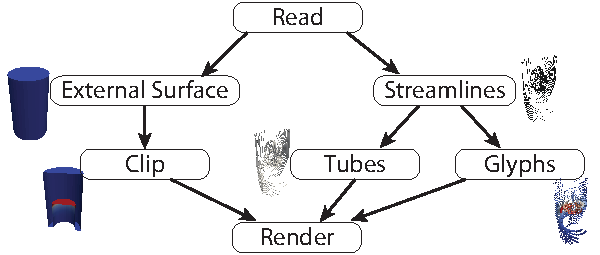
\includegraphics{images/BranchingPipeline} &
    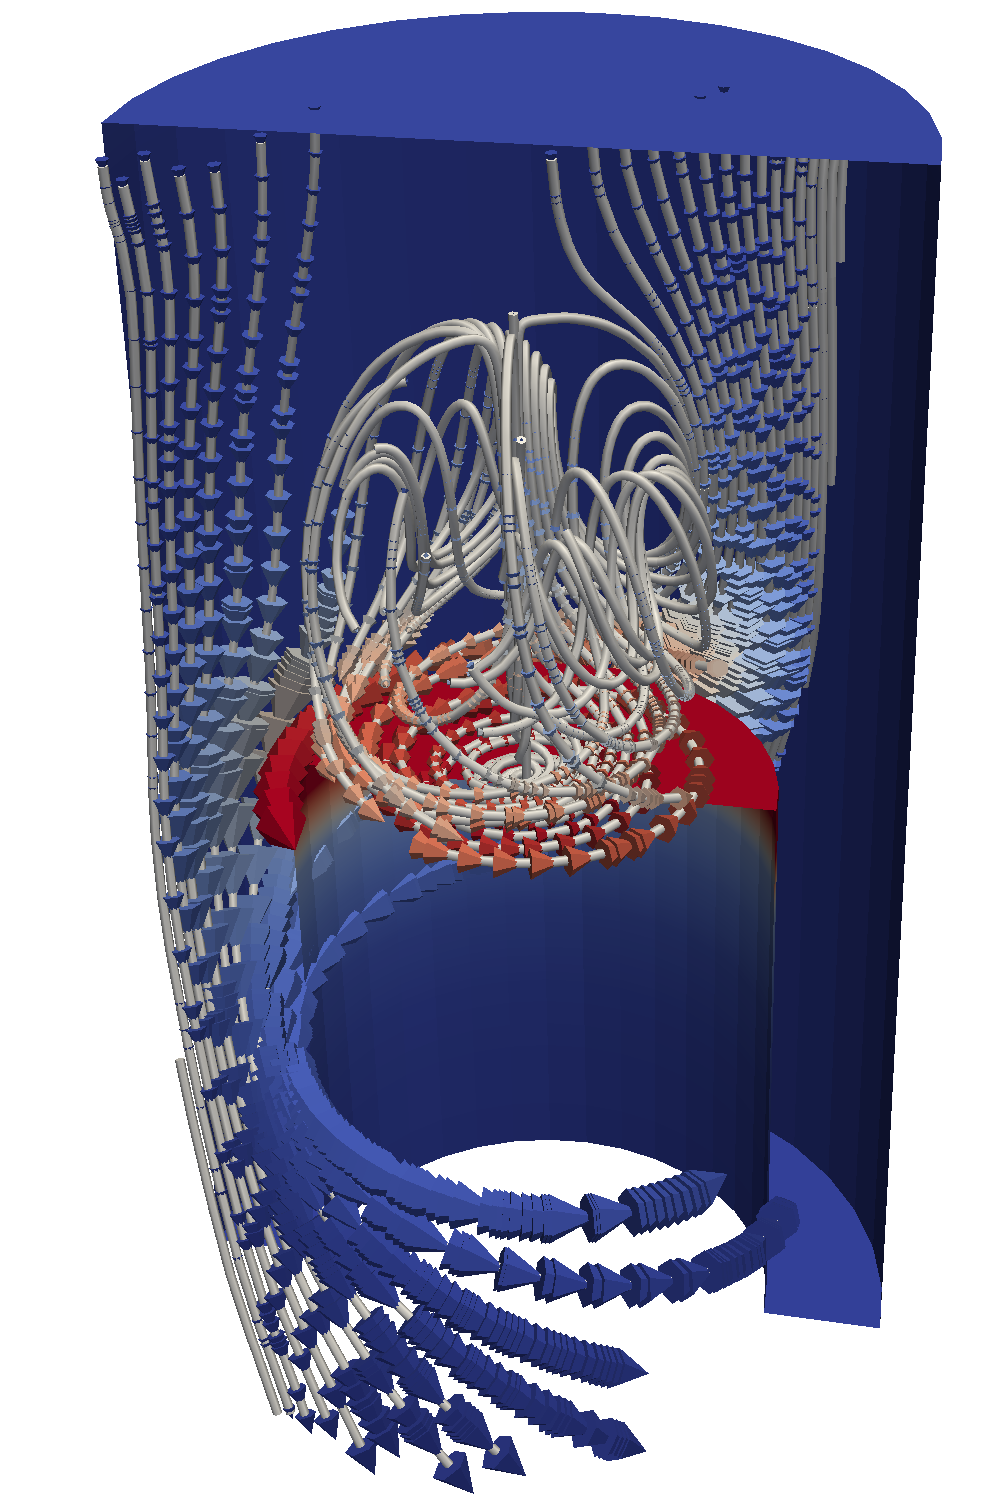
\includegraphics[height=1.7in]{images/BranchingPipelineResult}
  \end{tabular}
  \caption{A visualization pipeline with branching.  The final
    visualization is shown to the right.}
  \label{fig:BranchingPipeline}
\end{figure}

For more information on using visualization pipelines and the components
they typically contain, consult the documentation for one of the numerous
libraries or applications using a visualization
pipeline\lcite{VTK,ParaView,ParaViewTutorial,SCIRunUserGuide,IRISExplorerUsersGuide,VisTrailsDocumentation,OpenDXGuide}.


\section{Execution Management}
\label{sec:ExecutionManagement}

The topology of a pipeline dictates the flow of data and places constraints
on the order in which components can be executed, but it does not determine
how or when components get executed.  Visualization pipeline systems can
vary significantly in how they manage execution.

\subsection{Execution Drivers}
\label{sec:ExecutionDrivers}

The visualization pipeline represents a static network of operations
through which data flows.  Typical usage entails first establishing the
visualization pipeline and then executing the pipeline on one or more data
collections.  Consequently, the behavior of when components get executed is
a primary feature of visualization pipeline systems.  Visualization
pipelines generally fall under two execution systems: event driven and
demand driven.

An \keyterm{even-driven} pipeline launches execution as data becomes
available in sources.  When new data becomes available in a source, that
source component must be alerted.  When sources produce data, they push it
to the downstream components and trigger an event to execute them.  Those
downstream components in turn may produce their own data to push to the
next component.  Because the method of the event-driven pipeline is to push
data to the downstream components, this method is also known as the
\keyterm{push model}.  The event-driven method of execution is useful when
applying a visualization pipeline to data that is expected to change over
time.

A \keyterm{demand-driven} pipeline launches execution in response to
requests for data.  Execution is initiated at the bottom of the pipeline in
a sink.  The sink's upstream components satisfy this request by first
requesting data from their upstream components, and so on up to the
sources.  Once execution reaches a source, it produces data and returns
execution back to its downstream components.  The execution eventually
unrolls back to the originating sink.  Because the method of the
demand-driven pipeline is to pull data from the upstream components, this
method is also known as the \keyterm{pull model}.  The demand-driven method
of execution is useful when using a visualization pipeline to provide data
to an end system.  For example, the visualization could respond to render
requests to update a GUI.

\subsection{Caching Intermediate Values}
\label{sec:Caching}

Caching, which saves component execution outputs, is an important feature
for both execution methods.  In the case of the event-driven pipeline, a
component may execute only when data from all inputs is pushed to it.
Thus, the execution must know when to cache the data and where to retrieve
it when the rest of the data is later pushed.

In the case of the demand-driven pipeline, a component with fan out could
receive pull requests from multiple downstream components during the same
original sink request.  Rather than execute multiple times, the component
can first check to see if the previously computed result is still valid and
return that if possible.

Although caching all the intermediate values in a pipeline can remove
redundant computation, it also clearly requires more storage.  Thus,
managing the caching often involves a trade-off between speed and memory.
The cost of caching can be mitigated by favoring shallow copies of data
from a component's inputs to its outputs.

\subsection{Centralized vs. Distributed Control}
\label{sec:CentralizedDistributed}

The control mechanism for a visualization pipeline can be either
centralized or distributed.  A \keyterm{centralized control} has a single
unit managing the execution of all components in the pipeline.  The
centralized control has links to all components, understands their
connections, and initiates all execution in the pipeline.

A \keyterm{distributed control} has a separate unit for each component in
the pipeline.  The distributed control unit nominally knows only about a
single component and its inputs and outputs.  The distributed control unit
can initiate execution on only its own component and must send messages to
propagate execution elsewhere.

Centralized control is advantageous in that it can perform a more
thorough analysis of the pipeline's network to more finely control the
execution.  Such knowledge can be useful in making decisions about caching
(described in Section~\ref{sec:Caching}) and load balancing for parallel
execution (described in Section~\ref{sec:ParallelExecution}).  However, the
implementation of a centralized control is more complex because of the
larger management task.  Distributed control, in contrast, has more limited
knowledge of the pipeline, but tends to be simpler to implement and
manage.

\subsection{Interchangeable Executive}
\label{sec:InterchangeableExecutive}

Many visualization pipeline implementations have a fixed execution
management system.  However, such a system can provide more flexibility by
separating its execution management into a \keyterm{executive} object.  The
executive object is an independent object that manages pipeline execution.
Through polymorphism, different types of execution models can be
supported.  For example, VTK is designed as a demand-driven pipeline, but
with its interchangeable executives it can be converted to an event-driven
pipeline, as demonstrated by Vo \etal\scite{Vo2010}.

Replacing the executive in a pipeline with centralized control is
straightforward.  The control is, by definition, its own separate unit.  In
contrast, a distributed control system must have an independent executive
object attached to each component in the pipeline.  The component objects
get relegated to only a function to execute whereas the executive manages
pipeline connections, data movement, and execution\lcite{VTKUsersGuide}.

\subsection{Out-of-Core Streaming}
\label{sec:OutOfCore}

An \keyterm{out-of-core} algorithm (or more formally an
\keyterm{external-memory algorithm}) is a general algorithmic technique
that can be applied when a data set is too large to fit within a computer's
internal memory.  When processing data out of core, only a fraction of the
data is read from storage at any one time\lcite{Vitter2001}.  The results
for that region of data are generated and stored, then the next segment of
data is read.

A rudimentary but effective way of performing out-of-core processing in a
visualization pipeline is to read data in pieces and let each piece flow
through the pipe independently.  Because pieces are fed into the pipeline
sequentially, this method of execution is often called \keyterm{streaming}.
Streaming can only work on certain algorithms.  The algorithms must be
\keyterm{separable} (that is, can break the work into pieces and work on
one piece at a time), and the algorithms must be \keyterm{result invariant}
(that is, the order in which pieces are processed does not matter).  In a
demand-driven pipeline, it is also necessary that the algorithm is
\keyterm{mappable} in that it is able to identify what piece of input is
required to process each piece of output\lcite{Law1999}.

Because the input data set is broken into pieces, the boundary between
pieces is important for many algorithms.  Boundaries are often handled by
adding an extra layer of cells, called \keyterm{ghost
  cells}\lcite{Ahrens2001}.  These ghost cells complete the neighborhood
information for each piece and can be removed from the final result.

Some algorithms can be run out-of-core with a simple execution model that
iterates over pieces.  However, most pipelines can implement streaming more
effectively with metadata, discussed in Section~\ref{sec:Metadata}.

\subsection{Block Iteration}
\label{sec:BlockIteration}

Some data sets are actually a conglomerate of smaller data sets.  These
smaller data sets are called either \keyterm{blocks} or \keyterm{domains}
of the whole.  One example of a multi-block data set is an assembly of
parts.  Another example is adaptive mesh refinement (AMR)\lcite{Berger1989}
in which a hierarchy of progressively finer grids selectively refines
regions of interest.

Many visualization algorithms can be applied independently to each block in
a multi-block data set.  Rather than have every component specifically
attend to the multi-block nature of the data, the execution management can
implicitly run an algorithm independently on every block in the data
set\lcite{VTKUsersGuide}.


\section{Metadata}
\label{sec:Metadata}

So far, we have considered the visualization pipeline as simply a flow
network for data, and the earliest implementations were just that.  Modern
visualization pipelines have introduced the concept of metadata, a brief
description of the actual data, into the pipeline.  The introduction of
metadata allows the pipeline to process data in more powerful ways.
Metadata can flow through the pipeline independent of, and often in
different directions than, the actual data.  The introduction of metadata
can in turn change the execution management of the pipeline.

\subsection{Regions}
\label{sec:Regions}

Perhaps the most important piece of information a visualization pipeline
can use is the region the data is defined over and the regions the data can
be split up into.  Knowing and specifying regions supports execution
management for out of core and parallel computation (described in Sections
\ref{sec:OutOfCore} and \ref{sec:ParallelExecution}, respectively).

Visualization pipelines operate on three basic types of regions.
\begin{packeddescription}
\item[Extents] are valid index ranges for regular multidimensional arrays
  of data.  Extents allow a fine granularity in defining regions as
  sub-arrays within a larger array.
\item[Pieces] are arbitrary collections of cells.  Pieces allow
  unstructured grids to be easily decomposed into discretionary regions.
\item[Blocks] (or domains) represent a logical domain decomposition.
  Blocks are similar to pieces in that they can represent arbitrary
  collections, but blocks are defined by the data set and their structures
  are considered to have some meaning.
\end{packeddescription}
The region metadata may also include the spatial range of each region.
Such information is useful when performing operations with known spatial
bounds.

Region metadata can flow throughout the pipeline independently of data.  A
general implementation to propagate region information and select regions
requires the three pipeline passes demonstrated in
Figure~\ref{fig:RegionPasses}\lcite{Ahrens2001}.

\begin{figure}[htbp]
  \centering
  \begin{tabular}{@{}c@{\qquad}c@{\qquad}c@{}}
  \subfloat[Update Information]{
    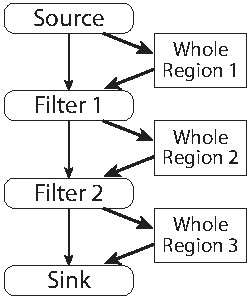
\includegraphics{images/UpdateInformation}
    \label{fig:RegionPasses:UpdateInformation}
  } &
  \subfloat[Update Region]{
    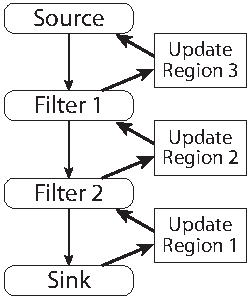
\includegraphics{images/UpdateRegion}
    \label{fig:RegionPasses:UpdateRegion}
  } &
  \subfloat[Update Data]{
    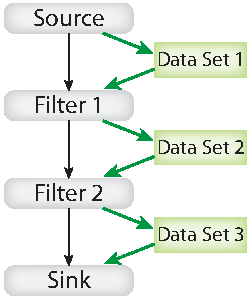
\includegraphics{images/UpdateData}
    \label{fig:RegionPasses:UpdateData}
  }
  \end{tabular}
  \caption{The three pipeline passes for using regional data.}
  \label{fig:RegionPasses}
\end{figure}

In the first \keyterm{update information} pass, sources produce the entire
region they can generate, and that region gets passed down the pipeline.
As the region passes through filters, they have the opportunity to change
the region.  This could be because the filter is combining multiple regions
from multiple inputs.  It could also be because the filter is generating a
new topology, which has its own independent regions.  It could also be
because the filter transforms the data in space or removes data from a
particular region in space.

In the second \keyterm{update region} pass, the application decides what
region of data it would like a sink to process.  This update region is then
passed backward up the pipeline during which each filter transforms the
region respective of the output to a region respective of the input.  The
update region pass terminates at the sources, which receive the region of
data they must produce.

In the final \keyterm{update data} pass, the actual data flows through the
pipeline as described in Section~\ref{sec:ExecutionManagement}.

\subsection{Time}
\label{sec:Time}

Until recently, visualization pipelines operated on data at a single
snapshot in time.  Operating on data that evolved over time entailed an
external mechanism executing the pipeline repeatedly over a sequence of
time steps.  Such behavior arose from data sets being organized as a
sequence of time steps and the abundance of visualization algorithms that
are time invariant.

Time control can be added the visualization pipeline by adding time
information to the metadata\lcite{Biddiscombe2007}.  The basic approach is
to add a time dimension to the region metadata described in
Section~\ref{sec:Regions}.  A source declares what time steps are
available, and each filter has the ability to augment that time during the
update information pass.  Likewise in the update region pass each filter
may request new or different time steps.  The region request may contain
one or more time steps.

These temporal regions enable filters that operate on data that changes
over time.  For example, a temporal interpolator filter can estimate
continuous time by requesting multiple time steps from upstream and
interpolating the results for downstream components.

Some algorithms, such as particle tracing, may need all data over all time.
Although such a region may be requested by this mechanism, it is seldom
feasible to load this much data at one time.  Instead, an algorithm may
operate on a small number of time steps at one time, iterate over all time,
and accumulate the results.  To support this, Biddiscombe
\etal\scite{Biddiscombe2007} propose a \keyterm{continue executing} mode
where a filter, while computing data, can request a re-execution of the
upstream pipeline with different time steps and then continue to compute
with the new data.

\subsection{Contracts}
\label{sec:Contracts}

Contracts\lcite{Childs2005} provide a generalized way for a filter to report
its \keyterm{impact}, the required data and operating modes, before the
filter processes data.  An impact may include the regions, variables, and
time step a filter expects to work on.  The impact might also include
operating restrictions such as whether the filter supports streaming or
requires ghost cells.

Filters declare their impact by modifying a \keyterm{contract} object.  The
contract is a data structure containing information about all the potential
meta-information the pipeline executive can use to manage execution.  The
contract object is passed up the pipeline in the same way an update region
would be passed up as depicted in
Figure~\ref{fig:RegionPasses:UpdateRegion}.  As the contract moves up the
pipeline, filters add their impacts to it, forming a union of the
requirements, abilities, and limitations of the pipeline.

\subsection{Prioritized Streaming}
\label{sec:PrioritizedStreaming}

The discussion of streaming in Section~\ref{sec:OutOfCore} provides no
scheme for the order in which pieces are processed.  In fact, since
streaming specifically requires a data invariant algorithm, the order of
operation is inconsequential with respect to correctness once the
processing is completed.

However, if one is interested in the intermediate results, the order is
consequential.  An interactive application may show the results of a
streaming visualization pipeline as they become available.  Such an
application can be improved greatly by prioritizing the streamed regions to
process those that provide the most information first\lcite{Ahrens2007}.
Possible priority metrics include the following.
\begin{packeditemize}
\item Regions in close proximity to the viewer in a three dimensional
  rendering should have higher priority.  Close objects are likely to
  obscure those behind.
\item Regions least likely to be culled should have the highest priority.
  Only objects within a certain frustum are visible in a three dimensional
  rendering, and some filters may remove data from particular spatial
  regions.
\item Regions with scalar values in an ``interesting'' range should be
  given priority.  Rendering parameters may assign an opacity to scalar
  values, and higher opacity indicates a greater interest.
\item Regions with more variability in a field may have higher priority.
  Homogeneous regions are unlikely to be interesting.
\end{packeditemize}

Prioritized streaming can become even more effective when the data contains
a hierarchy of resolutions\lcite{Ahrens2009}.  The highest priority is
given to the most coarse representation of the mesh.  This representation
provides a general overview visualization that can be immediately useful.
Finer sub-regions are progressively streamed in with the aforementioned
priorities.

\subsection{Query-Driven Visualization}
\label{sec:QueryDrivenVisualization}

\keyterm{Query-driven visualization} enables one to analyze a large data
set by identifying ``interesting'' data that matches some specified
criteria\lcite{Stockinger2005,Gosink2008}.  The technique is based off the
ability to quickly load small selections of data with arbitrary
specification.  This ability provides a much faster iterative analysis than
the classical analysis of loading large domains and sifting through the
data.  Performing query-driven visualization in a pipeline requires three
technologies: file indexing, a query language, and a pipeline metadata
mechanism to pass a query from sink to source.

Visualization queries rely on fast retrieval of data that matches the
query.  Queries can be based on combinations of numerous fields.  Thus, the
pipeline source must be able to identify where the pertinent data is
located without reading the entire file.  Although tree-based approaches
have been proposed\lcite{Chiang1998}, indexing techniques like
FastBit\lcite{FastBit,Wu2010} are most effective because they can handle an
arbitrary amount of dimensions.

A user needs a language or interface with which to specify a query.
Stockinger \etal\scite{Stockinger2005} propose compound Boolean expressions
such as all regions where $(\mathrm{temperature} > 1000\mathrm{K}) \;
\mathrm{AND} \; (70\mathrm{kPa} < \mathrm{pressure} < 90\mathrm{kPa})$.
Others add to the query capabilities with file-globbing like
expressions\lcite{Glatter2008} and predicate-based
languages\lcite{Johnson2009}.

Finally, the visualization pipeline must pass the query from the sink to
the source.  This is done by expanding either region metadata
(Section~\ref{sec:Regions}) or contracts (Section~\ref{sec:Contracts}) to
pass and adjust the field ranges in the query\lcite{Rubel2008}.


\section{Parallel Execution}
\label{sec:ParallelExecution}

Scientific visualization has a long history of using high performance
parallel computing to handle large-scale data.  Visualization pipelines
often encompass parallel computing capabilities.

\subsection{Basic Parallel Execution Modes}
\label{sec:ParallelExecution:Modes}

The most straightforward way to implement concurrency in a visualization
pipeline is to modify the execution control to execute different components
in the pipeline concurrently.  There are three basic modes to concurrent
pipeline scheduling: task, pipeline, and data\lcite{Ahrens2000}.

\subsubsection{Task Parallelism}
\label{sec:TaskParallelism}

\keyterm{Task parallelism} identifies independent portions of the pipeline
and executes them concurrently.  Independent parts of the pipeline occur
where sources produce data independently or where fan out feeds multiple
components.

\begin{figure}[htbp]
  \centering
  \begin{tabular}{@{}c@{\qquad}c@{\qquad}c@{}}
    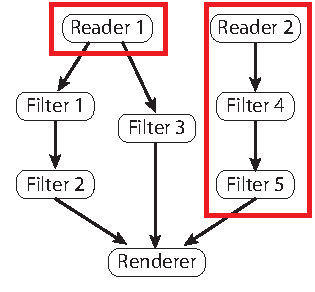
\includegraphics[scale=.65]{images/TaskParallel0} &
    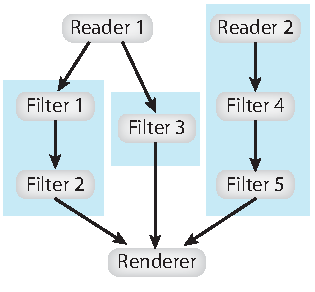
\includegraphics[scale=.65]{images/TaskParallel1} &
    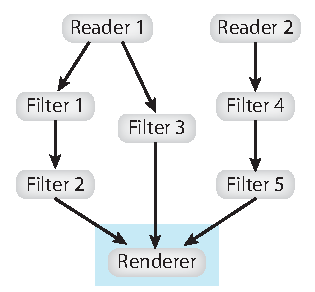
\includegraphics[scale=.65]{images/TaskParallel2} \\
    $T = t_0$ & $T = t_1$ & $T = t_2$
  \end{tabular}
  \caption{Concurrent execution with task parallelism.  Boxes indicate a
    region of the pipeline executed at a given time.}
  \label{fig:TaskParallelism}
\end{figure}

Figure~\ref{fig:TaskParallelism} demonstrates task parallelism applied to
an example pipeline.  At time $t_0$ the two readers begin executing
concurrently.  Once the first reader completes, at time $t_1$, both of its
downstream components may begin executing concurrently.  The other reader
and its downstream components may continue executing at this time, or they
may sit idle if they have completed.  After all of its inputs complete, at
time $t_2$, the renderer executes.

Because task parallelism breaks a pipeline into independent sub-pipelines
to execute concurrently, task parallelism can be applied to any type of
algorithm.  However, there are practical limits on how much concurrency
can be achieved with task parallelism.  Visualization pipelines in real
working environments can seldom be broken into more than a handful of
independent sub-pipelines.  Load balancing is also an issue.  Concurrently
running sub-pipelines are unlikely to finish simultaneously.

\subsubsection{Pipeline Parallelism}
\label{sec:PipelineParallelism}

\keyterm{Pipeline parallelism} uses streaming to read data in pieces and
executes different components of the pipeline concurrently on different
pieces of data.  Pipeline parallelism is related to out-of-core processing
in that a pipeline component is processing only a portion of the data at
any one time, but in the pipeline-parallelism approach multiple pieces are
loaded so that a component can process the next piece while downstream
components process the proceeding one.

\begin{figure}[htbp]
  \centering
  \begin{tabular}{@{}c@{\qquad}c@{\qquad}c@{\qquad}c@{}}
    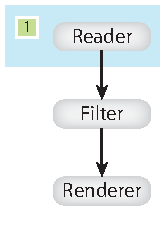
\includegraphics[scale=.65]{images/PipelineParallel0} &
    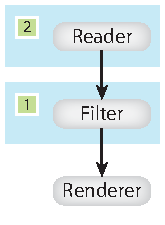
\includegraphics[scale=.65]{images/PipelineParallel1} &
    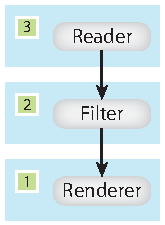
\includegraphics[scale=.65]{images/PipelineParallel2} &
    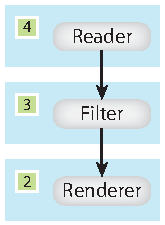
\includegraphics[scale=.65]{images/PipelineParallel3} \\
    $T = t_0$ & $T = t_1$ & $T = t_2$ & $T= t_3$
  \end{tabular}
  \caption{Concurrent execution with pipeline parallelism.  Boxes indicate
    a region of the pipeline executed at a given time with the piece number
    annotated.}
  \label{fig:PipelineParallelism}
\end{figure}

Figure~\ref{fig:PipelineParallelism} demonstrates pipeline parallelism
applied to an example pipeline.  At time $t_0$ the reader loads the first
piece of data.  At time $t_1$, the loaded piece is passed to the filter
where it is processed while the second piece is loaded by the reader.
Processing continues with each component working on the available piece
while the upstream components work on the next pieces.

Pipeline parallelism enables all the components in the pipeline to be
running concurrently.  Thus, pipeline parallelism tends to exhibit more
concurrency than task parallelism, but the amount of concurrency is still
severely limited by the number of components in the pipeline, which is
rarely much more than ten in practice.  Load balancing is also an issue as
different components are seldom expected to finish in the same length of
time.  More compute intensive algorithms will stall the rest of the
pipeline.  Also, because pipeline parallelism is a form of streaming, it is
limited to algorithms that are separable, result invariant, and mappable,
as described in Section~\ref{sec:OutOfCore}.

\subsubsection{Data Parallelism}
\label{sec:DataParallelism}

\begin{figure}[htbp]
  \centering
  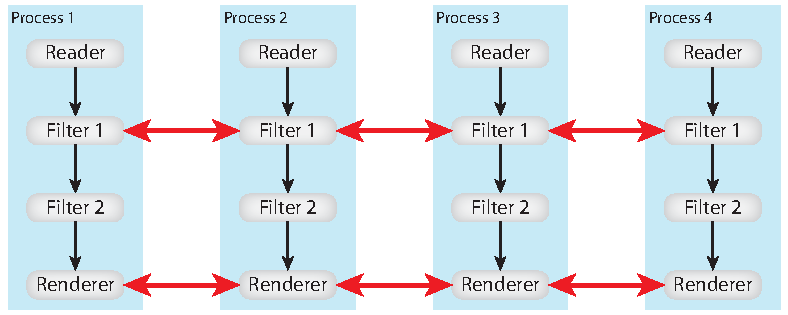
\includegraphics[scale=.65]{images/DataParallel}
  \caption{Concurrent execution with pipeline parallelism.  Boxes represent
    separate processes, each with its own partition of data.  Communication
    among processes may also occur.}
  \label{fig:DataParallelism}
\end{figure}

\keyterm{Data parallelism} partitions the input data into some set number
of pieces.  It then replicates the pipeline for each piece and executes
them concurrently, as shown in Figure~\ref{fig:DataParallelism}.

Of the three modes of concurrent scheduling, data parallelism is the most
widely used.  The amount of concurrency is limited only by the number of
pieces the data can be split into, and for large-scale data that number is
very high.  Data parallelism also works well on distributed-memory parallel
computers; data generally only needs to be partitioned once before
processing begins.  Data-parallel pipelines also tend to be well load
balanced; identical algorithms running on equal sized inputs tend to
complete in about the same amount of time.

Data parallelism is easiest to implement with algorithms that exhibit the
separable, result invariant, and mappable criteria of streaming execution.
In this case, the algorithm can be executed in data parallel mode with
little if any change.  However, it is possible to implement non-separable,
non-result-invariant algorithms with data parallel execution.  In this
case, the data-parallel pipelines must allow communication among the
processes executing a given component and the parallel executive must
ensure that all pipelines get executed simultaneously lest the
communication deadlock.  Common examples of algorithms that have special
data-parallel implementations are streamlines\lcite{Pugmire2009} and
connected components\lcite{Moreland2008:UltraVis}.  Data-parallel pipelines
also require special rendering for the partitioned data, which is described
in the following section.

Data-parallel pipelines are shown to be very scalable.  They have been
successfully ported to current
supercomputers\lcite{Moreland2008:CUG,Pugmire2008,Patchett2009} and have
demonstrated excellent parallel speedup\lcite{Childs2010,Moreland2010}.

\subsection{Rendering}
\label{sec:ParallelExecution:Rendering}

Data parallel pipelines, particularly those running on distributed-memory
parallel computers, require special consideration when rendering images,
which is often the sink operation in a visualization pipeline.  As in any
part of the data parallel pipeline, the rendering component does not have
complete access to the data.  Rather, the data is partitioned among a
number of replicated components.  In the case of rendering, this
component's processes must work together to form a single image from these
distributed data.

A straightforward approach is to collect the data to a single process and
render them serially\lcite{Miller1998,Johnson1999}.  This collection is
sometimes feasible when rendering surfaces because the surface geometry
tends to be significantly smaller than the volumes from which it is
derived.  However, geometry for large-scale data can still exceed a single
processor's limits, and the approach is generally impractical for volume
rendering techniques that require data for entire volumes.  Thus,
collecting data can become intractable.

A better approach is to employ a parallel rendering algorithm.
Data-parallel pipelines are most often used with a class of parallel
rendering algorithms called \keyterm{sort last}\lcite{Molnar1994}.
Sort-last parallel rendering algorithms are characterized by each process
first independently and concurrently rendering its local data into its own
local image and then collectively combining these locally generated images
into a single cohesive image.

Although it is possible to use other types of parallel rendering algorithms
with visualization pipelines\lcite{Moreland2003}, the properties of
sort-last algorithms make them most ideal for use in visualization
pipelines.  Sort-last rendering allows processes to render local data
without concern about the partitioning (although there are caveats
concerning transparent objects\lcite{Moreland2007}).  Such behavior makes
the rendering easy to adapt to whatever partition is created by the
data-parallel pipeline.  Also, the parallel overhead for sort-last
rendering is independent of the amount of data being rendered, and sort
last scales well with regard to the number of processes\lcite{Wylie2001}.
Thus, sort-last's parallel scalability matches the parallel scalability of
data-parallel pipelines.

\subsection{Hybrid Parallel}
\label{sec:HybridParallel}

Until recently, most high performance computers had distributed nodes with
each node containing some small amount of cores each.  These computers
could be effectively driven by treating each core as a distinct
distributed-memory process.

However, that trend is changing.  Current high performance computers now
typically have 8--12 cores per node, and that number is expected to grow
dramatically\lcite{ExascaleRoadMap,ASCACSummaryReport2010,ScientificDiscoveryExascale2011}.
When this many cores are contained in a node, it is often more efficient to
use \keyterm{hybrid parallelism} that considers both the distributed memory
parallelism among the nodes and the shared memory parallelism within each
node\lcite{Cappello2000}.  Recent development shows that pipeline
components with hybrid parallelism can out perform their corresponding
components considering each core as a separate distributed memory
node\lcite{Li2008,Camp2010,Howison2011}.

It should be noted that current implementations of hybrid parallelism are
not a feature of the visualization pipeline.  Rather, hybrid parallelism is
implemented by creating components with algorithms that perform shared
memory parallelism.  The data-parallel pipeline then provides distributed
memory parallelism on top of that.

\section{Miscellany}
\label{sec:Misc}

This section describes emerging features of visualization pipelines that do
not fit cleanly in any of the previous sections.

\subsection{Provenance}
\label{sec:Provenance}

Throughout this document we have considered the visualization pipeline as a
static thing that transforms data.  However, in real visualization
applications, the exploratory process involves making changes to the
visualization pipeline (i.e. adding and removing components or making
parameter changes).  It is therefore possible to model exploration as
transformations to the visualization pipeline\lcite{JankunKelly2002}.  This
\keyterm{provenance} of exploratory visualization can be captured and
exploited.

Provenance of pipeline transformations can assist exploratory visualization
in many ways.  Provenance allows users to quickly explore multiple
visualization methods and compare various parameter
changes\lcite{Bavoil2005}.  It also assists in reproducibility; because
provenance records the steps required to achieve a particular
visualization, it can be saved to automate the same visualization
later\lcite{Silva2007}.

Provenance information engenders the rare ability to perform analysis of
analysis, which allows for powerful supporting abilities.  Provenance
information can be compared and combined to provide revisioning information
for collaborative analysis tasks\lcite{Ellkvist2008}.  Provenance
information from previous analyses can be mined for future exploration.
Such data can be queried for apropos visualization
pipelines\lcite{Scheidegger2007} or used to automatically assist users in
their exploratory endeavors\lcite{Koop2008}.

\subsection{Scheduling on Heterogeneous Systems}
\label{sec:SchedulingHeterogeneous}

Computer architecture is rapidly moving to heterogeneous architecture.  GPU
units with general-purpose computing capabilities are already common, and
the use of similar accelerator units is likely to
grow\lcite{ExascaleRoadMap,ExascaleArchitecturesReport}.

Heterogeneous architectures introduce significant complications when
managing pipeline execution.  The algorithms in different pipeline
components may need to run on different types of processors.  If an
algorithm is capable of running on different types of processors, it will
have different performance characteristics on each one, which complicates
load balancing.

Furthermore, heterogeneous architectures typically have a more complicated
memory hierarchy.  For example, a CPU and GPU on the same system usually
have mutually inaccessible memory.  Even when memory is shared, there is
typically an \keyterm{affinity} to some section of memory, meaning that
data in some parts of memory can be accessed faster than data in other
parts of memory.  All this means that the pipeline execution must also
consider data location.

Hyperflow\lcite{VoPhD} is an emerging technology to address these issues.
Hyperflow manages parallel pipeline execution on heterogeneous systems.  It
combines all three modes of parallel execution (task, pipeline, and data
described in Section~\ref{sec:ParallelExecution:Modes}) along with
out-of-core streaming (described in Section~\ref{sec:OutOfCore}) to
dynamically allocate work based on thread availability and data location.

\fix{To my knowledge there is not yet a publication of hyperflow other than
  Huy's dissertation.  However, I'm sure Huy and Claudio are submitting it
  if it has not already been accepted.  Perhaps it will show up at IEEE
  Vis.}

\subsection{In Situ}
\label{sec:InSitu}


\section{Visualization Pipeline Alternatives}
\label{sec:Alternatives}

\subsection{Field Abstraction}
\label{sec:FieldAbstraction}

Field Model (FM).  Field Encapsulation Library (FEL).

\subsection{MapReduce}
\label{sec:MapReduce}

\subsection{Worklets}
\label{sec:Worklets}


\section{Conclusion}
\label{sec:Conclusion}


\section{Acknowledgments}

This work was supported in part by the DOE Office of Science, Advanced
Scientific Computing Research, under award number 10-014707, program
manager Lucy Nowell.

Sandia National Laboratories is a multi-program laboratory operated by
Sandia Corporation, a wholly owned subsidiary of Lockheed Martin
Corporation, for the U.S. Department of Energy's National Nuclear Security
Administration.

\bibliographystyle{plain}
\bibliography{VisPipelines}

\end{document}
